%Tipo de Documento [Conferencia]

\documentclass[conference]{IEEEtran}\usepackage[]{graphicx}\usepackage[]{color}
%% maxwidth is the original width if it is less than linewidth
%% otherwise use linewidth (to make sure the graphics do not exceed the margin)
\makeatletter
\def\maxwidth{ %
  \ifdim\Gin@nat@width>\linewidth
    \linewidth
  \else
    \Gin@nat@width
  \fi
}
\makeatother

\definecolor{fgcolor}{rgb}{0.345, 0.345, 0.345}
\newcommand{\hlnum}[1]{\textcolor[rgb]{0.686,0.059,0.569}{#1}}%
\newcommand{\hlstr}[1]{\textcolor[rgb]{0.192,0.494,0.8}{#1}}%
\newcommand{\hlcom}[1]{\textcolor[rgb]{0.678,0.584,0.686}{\textit{#1}}}%
\newcommand{\hlopt}[1]{\textcolor[rgb]{0,0,0}{#1}}%
\newcommand{\hlstd}[1]{\textcolor[rgb]{0.345,0.345,0.345}{#1}}%
\newcommand{\hlkwa}[1]{\textcolor[rgb]{0.161,0.373,0.58}{\textbf{#1}}}%
\newcommand{\hlkwb}[1]{\textcolor[rgb]{0.69,0.353,0.396}{#1}}%
\newcommand{\hlkwc}[1]{\textcolor[rgb]{0.333,0.667,0.333}{#1}}%
\newcommand{\hlkwd}[1]{\textcolor[rgb]{0.737,0.353,0.396}{\textbf{#1}}}%

\usepackage{framed}
\makeatletter
\newenvironment{kframe}{%
 \def\at@end@of@kframe{}%
 \ifinner\ifhmode%
  \def\at@end@of@kframe{\end{minipage}}%
  \begin{minipage}{\columnwidth}%
 \fi\fi%
 \def\FrameCommand##1{\hskip\@totalleftmargin \hskip-\fboxsep
 \colorbox{shadecolor}{##1}\hskip-\fboxsep
     % There is no \\@totalrightmargin, so:
     \hskip-\linewidth \hskip-\@totalleftmargin \hskip\columnwidth}%
 \MakeFramed {\advance\hsize-\width
   \@totalleftmargin\z@ \linewidth\hsize
   \@setminipage}}%
 {\par\unskip\endMakeFramed%
 \at@end@of@kframe}
\makeatother

\definecolor{shadecolor}{rgb}{.97, .97, .97}
\definecolor{messagecolor}{rgb}{0, 0, 0}
\definecolor{warningcolor}{rgb}{1, 0, 1}
\definecolor{errorcolor}{rgb}{1, 0, 0}
\newenvironment{knitrout}{}{} % an empty environment to be redefined in TeX

\usepackage{alltt}

%BIBLIOTECAS

% Este paquete se utiliza para generar texto o graficas de relleno.
%\usepackage{blindtext, graphicx}
%Biblioteca para graficas
\usepackage{graphicx}
%Biblioteca para lectura de caracteres ortográficos (tildes..etc. ) 
\usepackage[utf8]{inputenc}
%Biblioteca para enumeración de imagenes
\usepackage{float}
%Biblioteca para graficos vectrizados.svg 
\usepackage{svg}
\usepackage{enumerate}
%Biblioteca para enumerar figuras tablas.. etc en español 
\usepackage[spanish, es-tabla]{babel}
\usepackage[spanish]{babel}
%\usepackage[spanish,USenglish]{babel}

%INICIO DEL DOCUMENTO
\IfFileExists{upquote.sty}{\usepackage{upquote}}{}
\begin{document}
	
	
	% TITULO DEL PAPER
\title{Modelo predictivo para estimar el crecimiento poblacional hispano al a\~no 2020 en diferentes ciudades de EEUU}

% NOMBRE DE LOS AUTORES
\author{
	\IEEEauthorblockN{Leonel Muñoz Cedano}
	\IEEEauthorblockA{Ingeniero de Sistemas\\ 
		Universidad Distrital Francisco José de Caldas\\
		Bogotá D.C., Colombia\\
		Email: leoneling@gmail.com}
	%\and
}
%TITULO
\maketitle

%abstract del documento
\input{itemsDoc/abstract.tex}

%Iniciar Palabras Clave Formato IEEE
\begin{IEEEkeywords}
	Big Data, Data Mining, Dataset, Modelo predictivo, SMART.
\end{IEEEkeywords}

%Introduccion 
\input{itemsDoc/introduccion.tex}

%Metodologia
\input{itemsDoc/metodologia.tex}

%Preguntas de investigacion
\input{itemsDoc/QuestionsResearch.tex}
	
	% Analisis exploratorio

\section{Análisis exploratorio del DataSet}
El análisis exploratorio tiene como objetivo identificar el comportamiento de los datos a través del análisis estadístico. En este análisis se pueden visualizar en gran variaedad de tablas y gráficos que permitirán explorar las distribución de los datos e identificar comportamientos y/o características de las observaciones tales como; valores atípicos o outliers, concentraciones de valores, saltos o discontinuidades, forma de la distribución, etc.   



\subsection{Analisis inicial}
Lo primero que se va analizar es el comportamiento que tienen los datos en los diferentes años en las variables Total Población (TP), Total de Población no Hispana (TPNH) y Total de Población Hispana (TPH); donde se obtiene los siguientes resultados:
%\vspace{1mm}

% Table created by stargazer v.5.2 by Marek Hlavac, Harvard University. E-mail: hlavac at fas.harvard.edu
% Date and time: sáb, may 21, 2016 - 02:02:14 p.m.
\begin{table}[!htbp] \centering 
  \caption{Total de la población de EEUU} 
  \label{} 
\begin{tabular}{@{\extracolsep{5pt}}lccccc} 
\\[-1.8ex]\hline 
\hline \\[-1.8ex] 
Statistic & \multicolumn{1}{c}{N} & \multicolumn{1}{c}{Mean} & \multicolumn{1}{c}{St. Dev.} & \multicolumn{1}{c}{Min} & \multicolumn{1}{c}{Max} \\ 
\hline \\[-1.8ex] 
TP & 12,544 & 91,700.930 & 297,470.800 & 67 & 9,889,056 \\ 
TPNH & 12,544 & 78,932.380 & 214,518.700 & 60 & 5,511,922 \\ 
TPH & 12,544 & 12,768.550 & 102,278.800 & 0 & 4,760,974 \\ 
\hline \\[-1.8ex] 
\end{tabular} 
\end{table} 


%\vspace{1mm}
Es importante recordar que el anális principal de esta investigación se enfoca en estimar el crecimiento de la población hispana en las ciudades de EEUU, y analizando los resultados obtenidos de la variable TPH, se evidencia una media muy baja con respecto a los valores de máximo y mínimo de la misma.  Por tal razón se ha hace necesario visualizar el comportamiento de los datos de la variable TPH a través del siguiente gráfico.   
\vspace{-6mm}
\begin{figure}[H]
	\centering
\begin{knitrout}
\definecolor{shadecolor}{rgb}{0.969, 0.969, 0.969}\color{fgcolor}
\includegraphics[width=\maxwidth]{figure/conatipicos-1} 

\end{knitrout}
	\caption{Dotplot de la variable TPH}
\end{figure}
\vspace{-10mm}
En la gráfica anterior se observa la existencia de datos atípicos (outliers); los cuales distorsionan el análisis de la información y los resultados, por tal razón estas observaciones atípicas no serán tenidas en cuenta en el desarrollo del modelo predictivo.
\vspace{-6mm}
\begin{figure}[H]
	\centering
\begin{knitrout}
\definecolor{shadecolor}{rgb}{0.969, 0.969, 0.969}\color{fgcolor}
\includegraphics[width=\maxwidth]{figure/sinatipicos-1} 

\end{knitrout}
	\caption{Histograma de la variable TPH sin outliers}
\end{figure}

\vspace{-6mm}
\begin{figure}[H]
	\centering
\begin{knitrout}
\definecolor{shadecolor}{rgb}{0.969, 0.969, 0.969}\color{fgcolor}
\includegraphics[width=\maxwidth]{figure/sinatipicos2-1} 

\end{knitrout}
	\caption{Histograma de la variable PPH sin outliers}
\end{figure}
\vspace{-6mm}
Los histogramas obtenidos de las variables TPH y PPH expresan que las observaciones tienen un comportamiento exponencial, pero es muy temprano determinar cual será el tipo de modelo y la cantidad de variables a utilizar en el desarrollo de la predicción. A medida que se avance con el análisis de los datos y los resultados obtenidos en cada proceso se encargarán de determinar cual va ser el mejor modelo a aplicar en la investigación.        
\vspace{-6mm}
%\vspace{-3mm}
%\subsection{Analizando población hispana en el año 1990}
%Los datos más representativos se dan a continuación:
%%%<<media1990, results='asis'>>=
%%%	d1990 <- data.frame(TP=datos1990$TP,TPNH=datos1990$TPNH,TPH=datos1990$TPH)
%%%	stargazer(d1990,type="latex",title="Población de EEUU en el año 1990")
%%%@

%\vspace{-3mm}
%%%\begin{figure}[H]
%%%	\centering
%%%	<<pobHis1990,message=FALSE>>=
%%%	ggplot(datos1990,aes(TPH)) + geom_histogram()
%%%	@
%%%	\caption{Población Hispana en el año 1990}
%%%\end{figure}


%\vspace{-3mm}
%\subsection{Analizando población hispana en el año 2000}
%Los datos más representativos se dan a continuación:
%%%<<media2000, results='asis'>>=
%%%  d2000 <- data.frame(TP=datos2000$TP,TPNH=datos2000$TPNH,TPH=datos2000$TPH)
%%%  stargazer(d2000,type="latex",title="Población de EEUU en el año 2000")
%%%@

%\vspace{-5mm}
%%%\begin{figure}[H]
%%%	\centering
%%%	<<pobHisp2000,message=FALSE>>=
%%%	ggplot(datos2000,aes(TPH)) + geom_histogram()
%%%	@
%%%	\caption{Población Hispana en el año 2000}
%%%\end{figure}

%\vspace{-10mm}
%\subsection{Analizando población hispana en el año 2010}

%%%<<media2010, results='asis'>>=
%%%  d2010 <- data.frame(TP=datos2010$TP,TPNH=datos2010$TPNH,TPH=datos2010$TPH)
%%%  stargazer(d2010,type="latex",title="Población de EEUU en el año 2010")
%%%@


%\vspace{-10mm}
%\subsection{Analizando población hispana en el año 2011}
%Los datos más representativos se dan a continuación:

%%%<<media2011, results='asis'>>=
%%%  d2011 <- data.frame(TP=datos2011$TP,TPNH=datos2011$TPNH,TPH=datos2011$TPH)
%%%  stargazer(d2011,type="latex",title="Población de EEUU en el año 2011")
%%%@


%\vspace{-5mm}
%%%\begin{figure}[H]
%%%	\centering
%%%	<<pobHisp2010,message=FALSE>>=
%%%		ggplot(datos2010,aes(TPH)) + geom_histogram()
%%%	@
%%%	\caption{Población Hispana en el año 2010}
%%%\end{figure}


%\vspace{-10mm}
%%%\begin{figure}[H]
%%%	\centering
%%%	<<pobHisp2011,message=FALSE>>=
%%%		ggplot(datos2011,aes(TPH)) + geom_histogram()
%%%	@
%%%	\caption{Población Hispana en el año 2011}
%%%\end{figure}

%\vspace{-10mm}
\subsection{Percentiles del conjunto de datos}
El percentil de orden \(k\) es el cuantil de orden \(\dfrac {k} {100}\). El recorrido intercuantil refleja la variabilidad de las observaciones comprendidas entre los percentiles 25 y 75 en el conjunto de datos. En esta sesión se obtienen los percentiles del 25\%,  50\% y 75\% de las variables Total Población (TP), Total Población Hispana (TPH) y Total Población No Hispana (TPNH).

\vspace{-2mm}
% latex table generated in R 3.2.3 by xtable 1.8-2 package
% Sat May 21 14:02:16 2016
\begin{table}[ht]
\centering
\begin{tabular}{rrrr}
  \hline
 & PercentilesTP & PercentilesTPH & PercentilesTPNH \\ 
  \hline
25\% & 10514.00 & 146.00 & 9836.50 \\ 
  50\% & 23257.00 & 514.00 & 21826.00 \\ 
  75\% & 54200.50 & 2368.00 & 51145.00 \\ 
   \hline
\end{tabular}
\caption{Percentiles de TP, TPH y TPNH} 
\end{table}

\vspace{-6mm}

%\vspace{4mm}
%\begin{itemize}
%\item Percentiles del población en el año 1990
%%%	<<perc1990,results='asis',echo=FALSE, warning=FALSE, message=FALSE>>=
%%%		grupo1990TP <- c(quantile(datos1990$TP,c(.25)), quantile(datos1990$TP,c(.50)), quantile(datos1990$TP,c(.75)))
%%%		grupo1990PH <- c(quantile(datos1990$TPH,c(.25)), quantile(datos1990$TPH,c(.50)), quantile(datos1990$TPH,c(.75)))
%%%		grupo1990PNH <- c(quantile(datos1990$TPNH,c(.25)), quantile(datos1990$TPNH,c(.50)), quantile(datos1990$TPNH,c(.75)))
%%%		q1990<-data.frame(PercentilesTP=grupo1990TP, PercentilesTPH=grupo1990PH, PercentilesTPNH=grupo1990PNH)	 	
%%%	 	xtable(q1990,"Percentiles de TP, TPH y TPNH en el año 1990")
%%%	@

%%%	<<perc2000,results='asis',echo=FALSE, warning=FALSE, message=FALSE>>=
%%%		grupo2000TP <- c(quantile(datos2000$TP,c(.25)), quantile(datos2000$TP,c(.50)), quantile(datos2000$TP,c(.75)))
%%%		grupo2000PH <- c(quantile(datos2000$TPH,c(.25)), quantile(datos2000$TPH,c(.50)), quantile(datos2000$TPH,c(.75)))
%%%		grupo2000PNH <- c(quantile(datos2000$TPNH,c(.25)), quantile(datos2000$TPNH,c(.50)), quantile(datos2000$TPNH,c(.75)))
%%%		q2000<-data.frame(PercentilesTP=grupo2000TP, PercentilesTPH=grupo2000PH, PercentilesTPNH=grupo2000PNH)	 	
%%%		xtable(q2000,"Percentiles de TP, TPH y TPNH en el año 2000")
%%%	@
	
%%%	<<perc2010,results='asis',echo=FALSE, warning=FALSE, message=FALSE>>=
%%%		grupo2010TP <- c(quantile(datos2010$TP,c(.25)), quantile(datos2010$TP,c(.50)), quantile(datos2010$TP,c(.75)))
%%%		grupo2010PH <- c(quantile(datos2010$TPH,c(.25)), quantile(datos2010$TPH,c(.50)), quantile(datos2010$TPH,c(.75)))
%%%		grupo2010PNH <- c(quantile(datos2010$TPNH,c(.25)), quantile(datos2010$TPNH,c(.50)), quantile(datos2010$TPNH,c(.75)))
%%%		q2010<-data.frame(PercentilesTP=grupo2010TP, PercentilesTPH=grupo2010PH, PercentilesTPNH=grupo2010PNH)	 	
%%%		xtable(q2010,"Percentiles de TP, TPH y TPNH en el año 2010")
%%%	@
	
%%%	<<perc2011,results='asis',echo=FALSE, warning=FALSE, message=FALSE>>=
%%%		grupo2011TP <- c(quantile(datos2011$TP,c(.25)), quantile(datos2011$TP,c(.50)), quantile(datos2011$TP,c(.75)))
%%%		grupo2011PH <- c(quantile(datos2011$TPH,c(.25)), quantile(datos2011$TPH,c(.50)), quantile(datos2011$TPH,c(.75)))
%%%		grupo2011PNH <- c(quantile(datos2011$TPNH,c(.25)), quantile(datos2011$TPNH,c(.50)), quantile(datos2011$TPNH,c(.75)))
%%%		q2011<-data.frame(PercentilesTP=grupo2011TP, PercentilesTPH=grupo2011PH, PercentilesTPNH=grupo2011PNH)	 	
%%%		xtable(q2011,"Percentiles de TP, TPH y TPNH en el año 2011")
%%%	@
\vspace{-6mm}
\subsection{Matriz de coeficientes de correlación}
La matriz de coeficientes de correlación permite estudiar la relación o comportamiento que existe entre la variables del conjunto de datos. A continuación se muestra el resultado obtenido de la correlación: 

%Ciudad con menos población hispana en el año 2011
\vspace{-2mm}
% latex table generated in R 3.2.3 by xtable 1.8-2 package
% Sat May 21 14:02:16 2016
\begin{table}[ht]
\centering
\begin{tabular}{rrrrrr}
  \hline
 & TP & TPNH & TPH & PPH & AP \\ 
  \hline
TP & 1.00 & 1.00 & 0.65 & -0.03 & -0.01 \\ 
  TPNH & 1.00 & 1.00 & 0.61 & -0.06 & -0.02 \\ 
  TPH & 0.65 & 0.61 & 1.00 & 0.39 & 0.11 \\ 
  PPH & -0.03 & -0.06 & 0.39 & 1.00 & 0.12 \\ 
  AP & -0.01 & -0.02 & 0.11 & 0.12 & 1.00 \\ 
   \hline
\end{tabular}
\caption{Matriz de coeficientes de correlación} 
\end{table}

\vspace{-6mm}
\begin{figure}[H]
	\centering
\begin{knitrout}
\definecolor{shadecolor}{rgb}{0.969, 0.969, 0.969}\color{fgcolor}
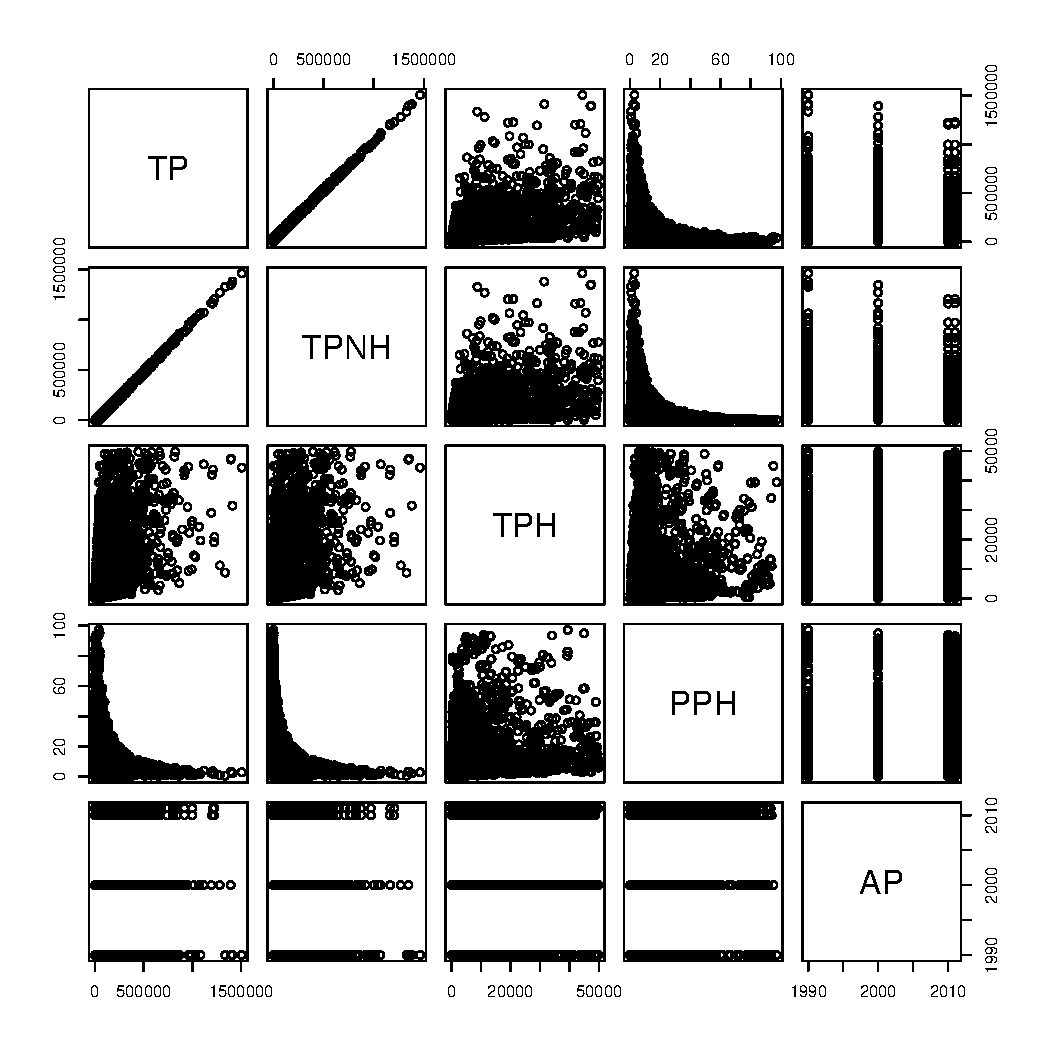
\includegraphics[width=\maxwidth]{figure/plotCor-1} 

\end{knitrout}
	\caption{Nube de puntos de correlación}
\end{figure}

El resultado de la matriz y nube de puntos de correlación, expresan la alta correlación de la variable TPH con respecto a las variables TP y TPNH.  Por otro lado, en la nube de puntos de correlación de la variable PPH, se evidencia un compotamiento exponencial con las variables TP y TPNH. 
	
	% Solución de preguntas



\section{Solución de Preguntas}
Han sido varios los resultados obtenidos hasta el momento, pero es necesario comenzar a dar respuesta a las diferentes preguntas que fueron planteadas al inicio de la investigación.

\subsection{Preguntas de caracter descriptivo}

%\begin{enumerate}
%A continuación se enumeran los promedios de la variable total ploblación en cada uno de los años del DataSet:
%\item los promedios por  año de los ciudadanos en EEUU, son los siguientes\\
%\begin{itemize}
%\item promedio del año 1990:
%<<unoa, results='asis', echo=FALSE, warning=FALSE, message=FALSE>>=
%	mean(datos1990$TP)
%@
%\item promedio del año 2000:
%<<unob,results='asis',echo=FALSE, warning=FALSE, message=FALSE>>=
%	mean(datos2000$TP)
%@
%\item promedio del año 2010:
%<<unoc,results='asis',echo=FALSE, warning=FALSE, message=FALSE>>=
%	mean(datos2010$TP)
%@
%\item promedio del año 2011:
%<<unod, results='asis', echo=FALSE, warning=FALSE, message=FALSE>>=
%	mean(datos2011$TP)
%@
%\end{itemize}

\begin{itemize}
  \item ¿Cuál es la Media de ciudadanos en EEUU durante los años  1990, 2000, 2010, 2011?
\end{itemize}

A continuación se enumeran las medias de la variables Total Población (TP), Total Población  No Hispana (TPNH) y Total Ploblación Hispana (TPH) en cada uno de los años del DataSet:

% latex table generated in R 3.2.3 by xtable 1.8-2 package
% Sat May 21 14:02:26 2016
\begin{table}[ht]
\centering
\begin{tabular}{rrrrr}
  \hline
 & Año 1990 & Año 2000 & Año 2010 & Año 2011 \\ 
  \hline
Media TP & 56941.88 & 58282.22 & 54864.33 & 55088.70 \\ 
  Media TPNH & 54998.83 & 55497.86 & 51221.69 & 51314.33 \\ 
  Media TPH & 1943.06 & 2784.35 & 3642.64 & 3774.37 \\ 
   \hline
\end{tabular}
\caption{Valores de las medias en TP, TPHN y TPH} 
\end{table}


\begin{itemize}
\item ¿Qué ciudad de EEUU tiene la mayor y menor población en el año 1990?
\end{itemize}

%\item Ciudad con más población en 1990
% latex table generated in R 3.2.3 by xtable 1.8-2 package
% Sat May 21 14:02:26 2016
\begin{table}[ht]
\centering
\begin{tabular}{rllr}
  \hline
 & Ciudad & Estado & Poblacion \\ 
  \hline
1 & King & Washington & 1507319 \\ 
   \hline
\end{tabular}
\caption{Ciudad con más población en el año 1990} 
\end{table}


%Ciudades con menos población en el año 1990
% latex table generated in R 3.2.3 by xtable 1.8-2 package
% Sat May 21 14:02:26 2016
\begin{table}[ht]
\centering
\begin{tabular}{rllr}
  \hline
 & Ciudad & Estado & Poblacion \\ 
  \hline
1 & Loving & Texas & 107 \\ 
   \hline
\end{tabular}
\caption{Ciudad con menos población en el año 1990} 
\end{table}


\begin{itemize}
\item ¿Qué ciudad de EEUU tiene la mayor y menor población en el año 2000?
\end{itemize}

%\item Ciudad con más población en 2000
% latex table generated in R 3.2.3 by xtable 1.8-2 package
% Sat May 21 14:02:26 2016
\begin{table}[ht]
\centering
\begin{tabular}{rllr}
  \hline
 & Ciudad & Estado & Poblacion \\ 
  \hline
1 & King & Washington & 1507319 \\ 
   \hline
\end{tabular}
\caption{Ciudad con más población en el año 2000} 
\end{table}


%Ciudades con menos población en el año 2000
% latex table generated in R 3.2.3 by xtable 1.8-2 package
% Sat May 21 14:02:26 2016
\begin{table}[ht]
\centering
\begin{tabular}{rllr}
  \hline
 & Ciudad & Estado & Poblacion \\ 
  \hline
1 & Loving & Texas &  67 \\ 
   \hline
\end{tabular}
\caption{Ciudad con menos población en el año 2000} 
\end{table}


\begin{itemize}
\item ¿Qué ciudad de EEUU tiene la mayor y menor población en el año 2010?
\end{itemize}


Ciudad de EEUU con la mayor población en el año 2010:
% latex table generated in R 3.2.3 by xtable 1.8-2 package
% Sat May 21 14:02:26 2016
\begin{table}[ht]
\centering
\begin{tabular}{rllr}
  \hline
 & Ciudad & Estado & Poblacion \\ 
  \hline
1 & Allegheny & Pennsylvania & 1223348 \\ 
   \hline
\end{tabular}
\caption{Ciudad con más población en el año 2010} 
\end{table}

\vspace{-6mm}
Ciudad de EEUU con la menor población en el año 2010

% latex table generated in R 3.2.3 by xtable 1.8-2 package
% Sat May 21 14:02:26 2016
\begin{table}[ht]
\centering
\begin{tabular}{rllr}
  \hline
 & Ciudad & Estado & Poblacion \\ 
  \hline
1 & Loving & Texas &  82 \\ 
   \hline
\end{tabular}
\caption{Ciudad con menos población en el año 2010} 
\end{table}


\begin{itemize}
\item ¿Qué ciudad de EEUU tiene la mayor y menor población en el año 2011?
\end{itemize}

%%%<<cinca, results='asis',echo=FALSE, warning=FALSE, message=FALSE>>=
%%%	ciudad5a <- subset(datos2011,datos2011$TP==max(datos2011$TP))
%%%	ciudad2011ta <- data.frame(Ciudad=ciudad5a$COUNTY, Estado=ciudad5a$STATE, Poblacion=ciudad5a$TP)
%%%	xtable(ciudad2011ta,"Ciudad con más población en el año 2011")
%%%@

%%%<<cincb, results='asis',echo=FALSE, warning=FALSE, message=FALSE>>=
%%%ciudad5b <- subset(datos2011,datos2011$TP==min(datos2011$TP))
%%%ciudad2011tb <- data.frame(Ciudad=ciudad5b$COUNTY, Estado=ciudad5b$STATE, Poblacion=ciudad5b$TP)  
%%%xtable(ciudad2011tb,"Ciudad con menos población en el año 2011")
%@

\begin{itemize}
\item ¿Cuál es el Promedio de ciudadanos hispanos en ciudades de EEUU en los años 1990, 2000, 2010 y 2011?
\end{itemize}

A continuación se enumera las medias de la variables Total Población (TP), Total Población  No Hispana (TPNH) y Total Ploblación Hispana (TPH) en cada uno de los años del DataSet:
\vspace{-1mm}
% latex table generated in R 3.2.3 by xtable 1.8-2 package
% Sat May 21 14:02:26 2016
\begin{table}[ht]
\centering
\begin{tabular}{rrrr}
  \hline
 & TP & TPNH & TPH \\ 
  \hline
1 & 56941.88 & 54998.83 & 1943.06 \\ 
  2 & 58282.22 & 55497.86 & 2784.35 \\ 
  3 & 54864.33 & 51221.69 & 3642.64 \\ 
  4 & 55088.70 & 51314.33 & 3774.37 \\ 
   \hline
\end{tabular}
\caption{Valores de las medias en TP, TPHN y TPH} 
\end{table}


%Ciudad con mas población hispana en el año 1990
%%%<<sieta,results='asis',echo=FALSE, warning=FALSE, message=FALSE>>=
%%%	ciudad7a <- subset(datos1990,datos1990$TPH==max(datos1990$TPH))
%%%	ciudad1990ha <- data.frame(Ciudad=ciudad7a$COUNTY, Estado=ciudad7a$STATE, PoblacionH=ciudad7a$TPH)
%%%	xtable(ciudad1990ha,"Ciudad con mayor TPH en el año 1990")
%%%@

%Ciudades con menos población hispana en el año 1990
%%%<<sietb,results='asis',echo=FALSE, warning=FALSE, message=FALSE>>=
%%%	ciudad7b <- subset(datos1990,datos1990$TPH==min(datos1990$TPH))
%%%	ciudad1990hb <- data.frame(Ciudad=ciudad7b$COUNTY, Estado=ciudad7b$STATE, PoblacionH=ciudad7b$TPH)  
%%%	xtable(ciudad1990hb,"Ciudad con menor TPH en el año 1990")
%%%@

%Ciudad con más población hispana en el año 2000
%%%<<ochoa,results='asis',echo=FALSE, warning=FALSE, message=FALSE>>=
%%%	ciudad8a <- subset(datos2000,datos2000$TPH==max(datos2000$TPH))
%%%	ciudad2000ha <- data.frame(Ciudad=ciudad8a$COUNTY, Estado=ciudad8a$STATE, PoblacionH=ciudad8a$TPH)
%%%	xtable(ciudad2000ha,"Ciudad con mayor TPH en el año 2000")
%%%@

%Ciudades con menos población hispana en el año 2000
%%%<<ochob,results='asis',echo=FALSE, warning=FALSE, message=FALSE>>=
%%%	ciudad8b <- subset(datos2000,datos2000$TPH==min(datos2000$TPH))
%%%	ciudad2000hb <- data.frame(Ciudad=ciudad8b$COUNTY, Estado=ciudad8b$STATE, Poblacion%%%H=ciudad8b$TPH)  
%%%	xtable(ciudad2000hb,"Ciudad con menor TPH en el año 2000")
%%%@

%Ciudad con más población hispana en el año 2010
%%%<<nueva,results='asis',echo=FALSE, warning=FALSE, message=FALSE>>=
%%%ciudad9a <- subset(datos2010,datos2010$TPH==max(datos2010$TPH))
%%%ciudad2010ha <- data.frame(Ciudad=ciudad9a$COUNTY, Estado=ciudad9a$STATE, PoblacionH%%%=ciudad9a$TPH)
%%%xtable(ciudad2010ha,"Ciudad con mayor TPH en el año 2010")
%%%@

%Ciudad con menos población hispana en el año 2010
%%%<<nuevb,results='asis',echo=FALSE, warning=FALSE, message=FALSE>>=
%%% 	ciudad9b <- subset(datos2010,datos2010$TPH==min(datos2010$TPH))
%%%  	ciudad2010hb <- data.frame(Ciudad=ciudad9b$COUNTY, Estado=ciudad9b$STATE, %%%PoblacionH=ciudad9b$TPH)
%%%  	xtable(ciudad2010hb,"Ciudad con menor TPH en el año 2010")
%%%@

%Ciudad con más población hispana en el año 2011
%%%<<diesa,results='asis',echo=FALSE, warning=FALSE, message=FALSE>>=
 %%%	ciudad10a <- subset(datos2011,datos2011$TPH==max(datos2011$TPH))
%%%  	ciudad2011ha <- data.frame(Ciudad=ciudad10a$COUNTY, Estado=ciudad10a$STATE, %%%PoblacionH=ciudad10a$TPH)
%%%  	xtable(ciudad2011ha,"Ciudad con mayor TPH en el año 2011")
%%%@

%Ciudad con menos población hispana en el año 2011
%%%<<diesb,results='asis',echo=FALSE, warning=FALSE, message=FALSE>>=
%%% 	ciudad10b <- subset(datos2011,datos2011$TPH==min(datos2011$TPH))
%%%	ciudad2011hb <- data.frame(Ciudad=ciudad10b$COUNTY, Estado=ciudad10b$STATE, %%%PoblacionH=ciudad10b$TPH)
%%% 	xtable(ciudad2011hb,"Ciudad con menor TPH en el año 2011")
%%%@

	
	%BIBLIOGRAFÍA
	%ENTORNO {thebibliography}
	%Permite al autor listar las referencias utilizadas y citarlas en algun punto del texto.
	
	\newpage
	 \begin{thebibliography}{1}
	 	
	 	\bibitem{biblio1}
	 	S. Mohanty, M. Jagadeesh and H. Srivatsa, Big Data Imperatives: Enterprise Big Data Warehouse, BI Implementations and Analytics, Published Apress, Isbn: 978-1-4302-4872-9, New York, 2013.
	 	
	 	\bibitem{biblio2}
	 	pewhispanic.org, Pew Research Center’s Hispanic Trends Project, U.S. Hispanic Population by County, 1980-2011. Disponible en: http://www.pewhispanic.org/2013/08/29/u-s-hispanic-population-by-county-1980-2011/, 2013.
	 	 	
	 	\bibitem{biblio3}
	 	G. T. Doran, There's a S.M.A.R.T. Way to Write Management's Goals and Objectives, Management Review, Vol. 70, Issue 11, pp. 35-36, 1981.
	 	
	 	\bibitem{biblio4}
	 	R. D. Peng and E. Matsui, The Art of Data Science: A guide for anyone who works whit data, Published Leanpub, Disponible en:http://leanpub.com/artofdatascience, 2015.
	 	 	
	 	\bibitem{biblio5}
	 	Alzate Marco, 250 Conceptos de Probabilidad, variables aleatorias y procesos estocásticos en redes de comunicaciones, Universidad Distrital Fransisco José de Caldas, pag 15-123, 2005.
	 	
 		\bibitem{biblio6}
 		G. C. Canavos, Probabilidad y estadística: Aplicaciones y métodos, Virginia Commonwealth University, Published McGRAW HILL, 1988.
	 	
	 \end{thebibliography}
	
\end{document}
